\chapter{Аналитический раздел}
В данном разделе будет проанализирована поставленная задача, определён необходимый функционал програмного обеспечения, описаны роли пользователей программы и будет произведён анализ существующих моделей базы данных.

\section{Постановка задачи}
Необходимо разработать программу для отображения информации интернет-магазина парфюмерии. Покупатель должен иметь возможность просмотра каталога товаров, оформления зазаза выбранной продукции, написания отзывов к заказанным товарам и постановки оценок товарам. Необходимо предусмотреть наличие ролей менеджера и администратора, осуществляющих управление продукцией, заказами и регулярующих деятельность покупателей.
\section{Формализация данных}

\begin{table}[h!]
	\begin{center}
		\caption{Данные и сведения о них}
		\begin{tabular}{ |p{5cm}|p{11cm}| }
			\hline
			\textbf{Данные} & \textbf{Сведения}\\ \hline
			Пользователь &  ФИО, дата рождения, адрес, e-mail, пароль, права доступа\\ \hline
			Товар &  Описание, фото, категория, количество, стоимость\\ \hline
			Заказ &  Товары, дата, стоимость, статус, комментарий\\ \hline
			Отзыв &  Содержание, дата, пользователь\\ \hline
			Оценка &  Дата, значение, пользователь\\ \hline
		\end{tabular}
		\label{data-table}
	\end{center}
\end{table}		

\newpage

\section{ER-диаграмма сущностей}

На рисунке \ref{er_diagram} представлена ER-диаграмма сущностей проекта.

\begin{figure}[h!]
	\begin{center}
		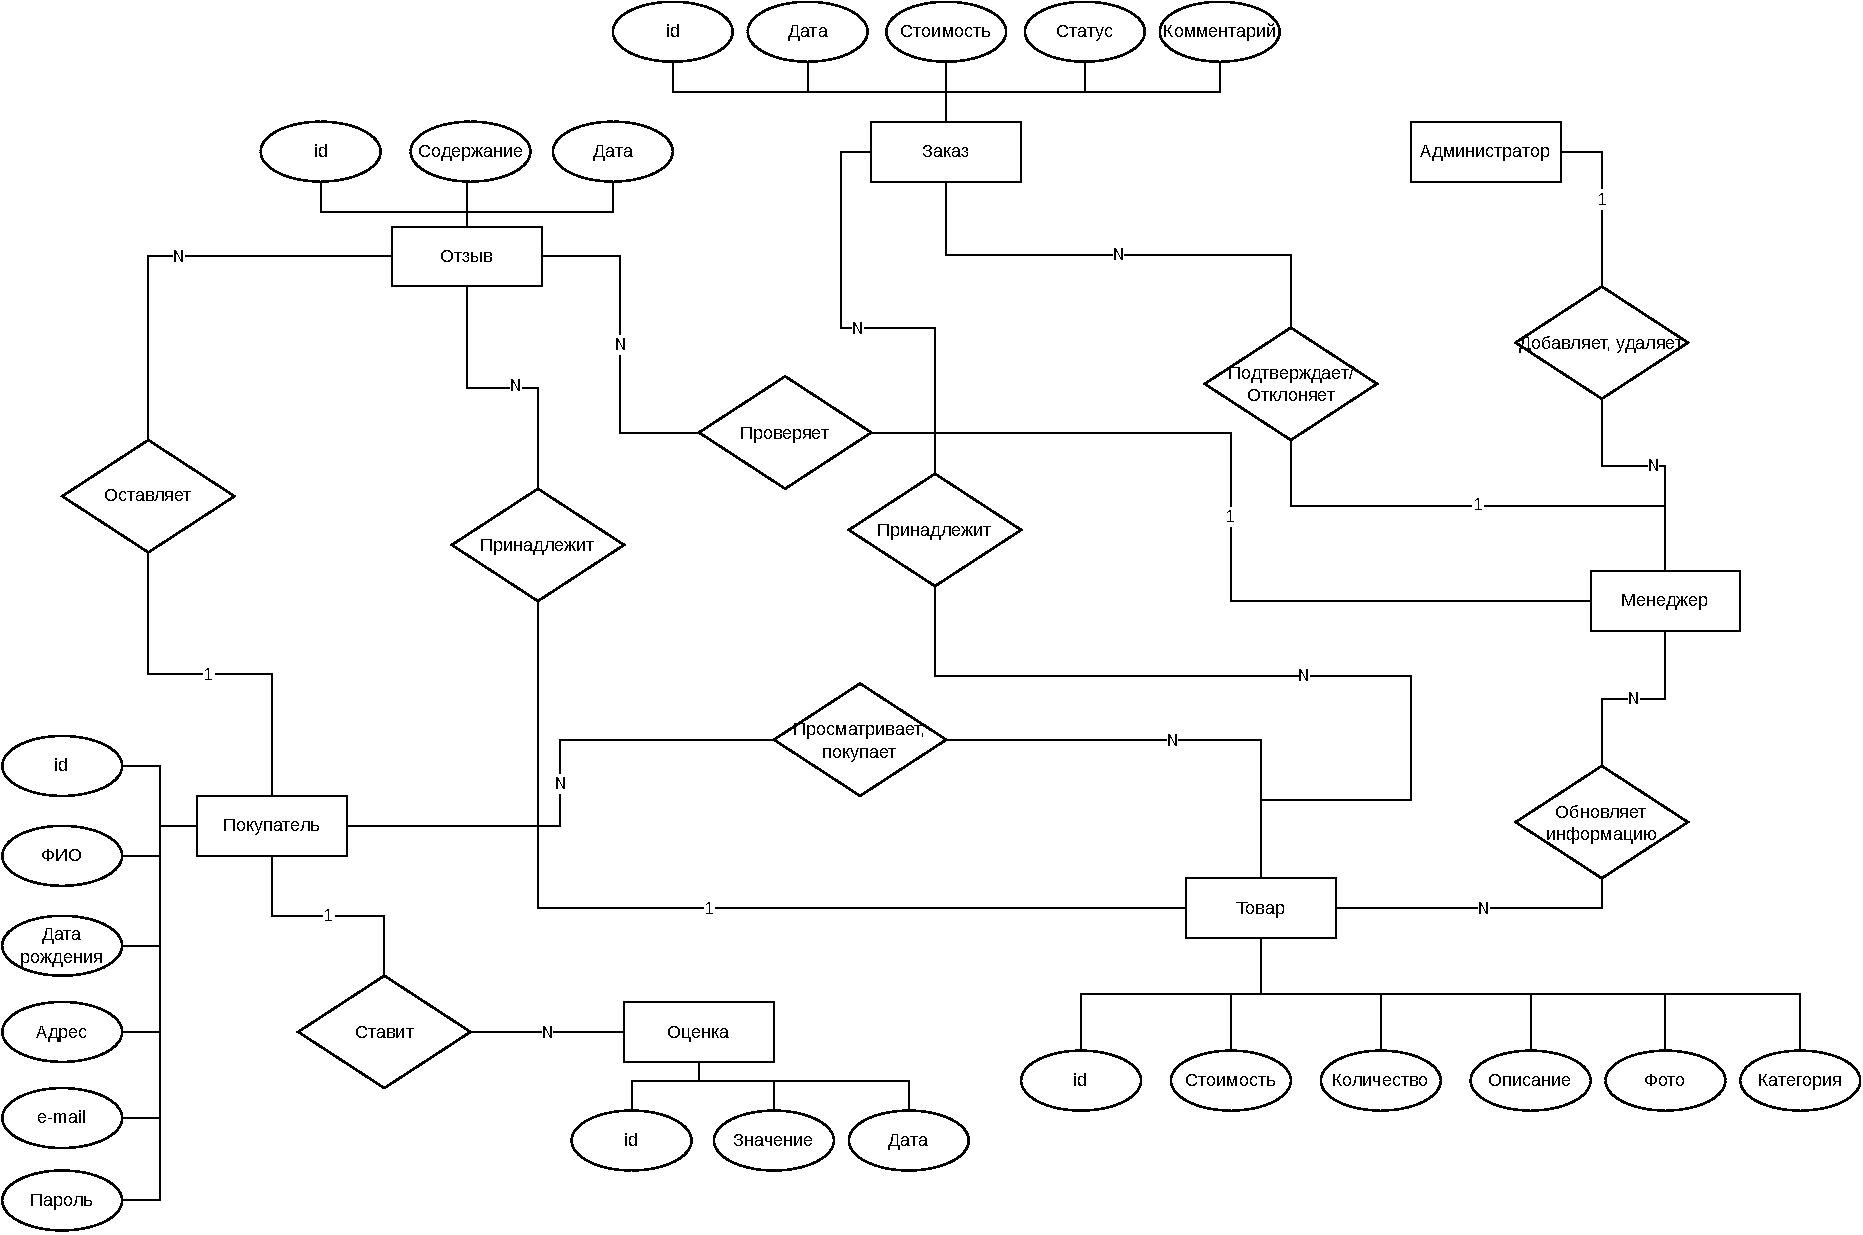
\includegraphics[scale=0.65, angle=90]{assets/er.pdf}
	\end{center}
	\caption{ER-диаграмма сущностей}
	\label{er_diagram}
\end{figure}

\section{Типы пользователей}

\begin{table}[h!]
	\begin{center}
		\caption{Типы пользователей и их функционал}
		\begin{tabular}{ |p{5cm}|p{11cm}| }
			\hline
			\textbf{Тип пользователя} & \textbf{Функционал}\\ \hline
			Покупатель & Просмотр каталога продукции и информации о товарах, написание отзывов и постановка оценок\\ \hline
			Менеджер & Просмотр каталога продукции и информации о товарах\newline Просмотр информации покупателей, просмотр информации о заказах, подтверждение и отклонение заказов, обновление продукции и информации о ней, модерация комментариев пользователей\\ \hline
			Администратор & Просмотр каталога продукции и информации о товарах\newline Просмотр информации покупателей, просмотр информации о заказах, подтверждение и отклонение заказов, обновление продукции и информации о ней, модерация комментариев пользователей\newline Добавление и удаление пользователей\\ \hline
		\end{tabular}
		\label{user-table}
	\end{center}
\end{table}		

\newpage

На рисунке \ref{use_case} представлена Use-Case-диаграмма.

\begin{figure}[h!]
	\begin{center}
		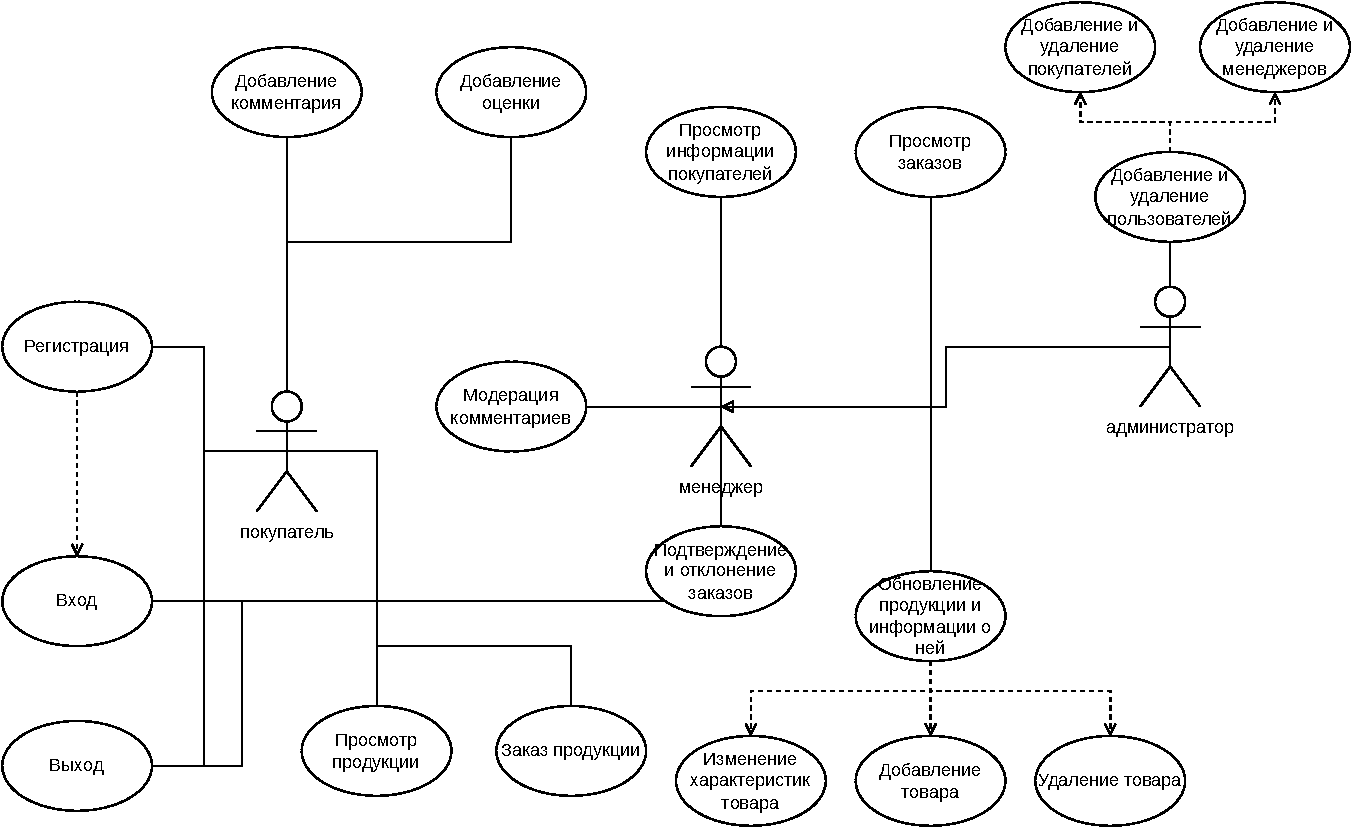
\includegraphics[scale=0.6]{assets/use_case.pdf}
	\end{center}
	\caption{Use-Case диаграмма}
	\label{use_case}
\end{figure}

\section{Описание существующих СУБД}
\textbf{Система управления базами данных} --- совокупность программных и лингвистических средств общего или специального назначения, обеспечивающих управление созданием и использованием баз данных.

\subsection{Основные функции СУБД}
Основынми функциями СУБД являются:
\begin{itemize}
	\item управление данными во внешней памяти;
	\item управление данными в оперативной памяти с использованием дискового кэша;
	\item журнализация изменений, резервное копирование и восстановление базы данных после сбоев;
	\item поддержка языков БД.
\end{itemize}

\subsection{Классификация СУБД по модели данных}
\textbf{Модель данных} --- это абстрактное, самодостаточное, логическое определение объектов, операторов и прочих элементов, в совокупности составляющих абстрактную машину доступа к данным, с которой взаимодействует пользователь. Эти объекты позволяют моделировать структуру данных, а операторы --- поведение данных. 

Существует 3 основных типа моделей организации данных:
\begin{itemize}
	\item иерархическая;
	\item сетевая;
	\item реляционная.
\end{itemize}

В иерархической модели данных используется представление базы данных в виде древовидной структуры, состоящей из объектов различных уровней. Между объектами существуют связи, каждый объект может включать в себя несколько объектов более низкого уровня. Такие объекты находятся в отношении предка к потомку, при этом возможна ситуация, когда объект-предок имеет несколько потомков, тогда как у объекта-потомка обязателен только один предок.

\begin{figure}[h!]
	\begin{center}
		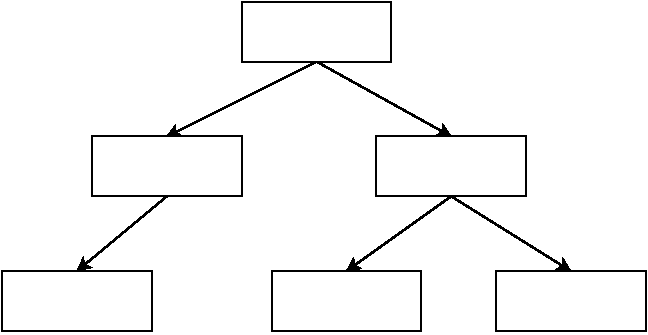
\includegraphics[scale=0.6]{assets/bd_scheme_1.pdf}
	\end{center}
	\caption{Cтруктура иерархической модели данных}
	\label{bd_scheme_1}
\end{figure}

В сетевой модели данных, в отличии от иерархической, у потомка может иметься любое число предков. Сетевая БД состоит из набора экземпляров определенного типа записи и набора экземпляров определенного типа связей между этими записями.
Главным недостатком сетевой модели данных являются жесткость и высокая сложность схемы базы данных, построенной на основе этой модели. Так как логика процедуры выбора данных зависит от физической организации этих данных, то эта модель не является полностью независимой от приложения. Иначе говоря, если будет необходимо изменить структуру данных, то нужно будет изменять и приложение.

\begin{figure}[h!]
	\begin{center}
		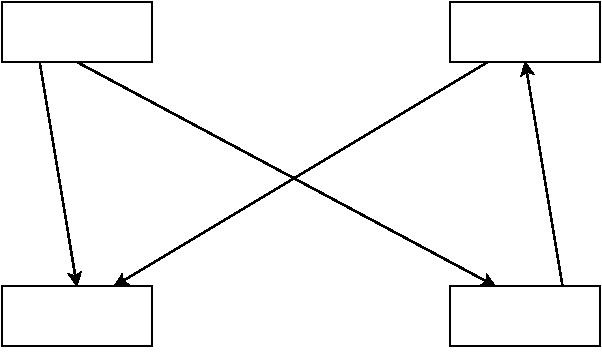
\includegraphics[scale=0.6]{assets/bd_scheme_2.pdf}
	\end{center}
	\caption{Cтруктура сетевой модели данных}
	\label{bd_scheme_2}
\end{figure}

Реляционная модель данных является совокупностью данных и состоит из набора двумерных таблиц. При табличной организации отсутствует иерархия элементов. Таблицы состоят из строк --- записей и столбцов --- полей. На пересечении строк и столбцов находятся конкретные значения. Для каждого поля определяется множество его значений. За счет возможности просмотра строк и столбцов в любом порядке достигается гибкость выбора подмножества элементов.


\begin{figure}[h!]
	\begin{center}
		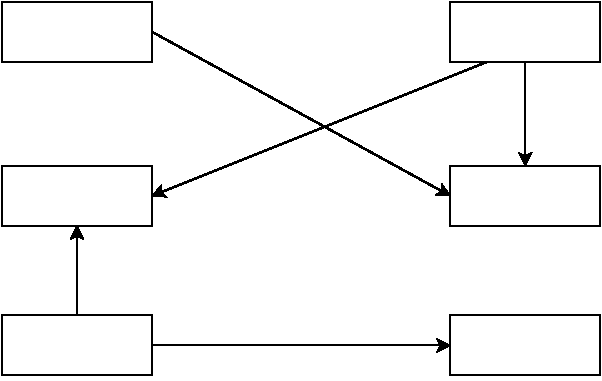
\includegraphics[scale=0.6]{assets/bd_scheme_3.pdf}
	\end{center}
	\caption{Cтруктура реляционной модели данных}
	\label{bd_scheme_3}
\end{figure}

\section*{Вывод}
\addcontentsline{toc}{section}{Вывод}

Поскольку реляционная модель базы данных является наиболее широко используемой и удобной, а также имеет возможность изменения базы данных без глобальных изменений программного обеспечения, то для реализации данного проекта была выброана именно она.

В данном разделе была произведена формализация поставленной задачи, описан необходимый функционал с распределением по ролям, проанализорованы модели базы данных и выбрана реляционная модель.